\section{Lecture 6: The Frequency Response}

We have seen that the output of a system is given from the
convolution of an input signal and the system's impulse response
%
\begin{displaymath}
  y(t) = x(t) * h(t) = \int\dx{\tau}x(\tau)h(t-\tau) \,.
\end{displaymath}
%
We have also seen from our study of the Fourier series that a
convolution in the time domain becomes a multiplication in the
frequency domain. We can show this holds for the Fourier transform
%
\begin{align*}
  Y(\omega) &= \int\dx{t} y(t)\ex{-\im\omega t}
  = \int\dx{t}\ex{-\im\omega t}\left[\int\dx{\tau}x(\tau)h(t-\tau)\right]
  = \int\dx{\tau}x(\tau)\left[\int\dx{t}h(t-\tau)\ex{-\im\omega t}\right] \\
  &= \int \dx{\tau}x(\tau)\mathscr{F}\left[h(t-\tau)\right] \,,
\end{align*}
%
where $\mathscr{F}$ denotes a Fourier transform. From the time-shifting
property of the Fourier transform established in the previous lecture,
this conveniently becomes
%
\begin{align*}
  Y(\omega) &= \int \dx{\tau}x(\tau)\mathscr{F}\left[h(t-\tau)\right]
  = \int \dx{\tau}x(\tau)H(\omega)\ex{-\im\omega\tau} \\
  &= \mathscr{F}\left[x(\tau)\right]H(\omega) = X(\omega)H(\omega) \,,
\end{align*}
%
as required.\\

From our earlier treatment of LTI systems, we know that the convolution
is important since the impulse response fully characterises the system.
The Fourier transform of this quantity, $H(\omega)$, is referred to as
the \textbf{frequency response}.

\subsection{What Does the Frequency Response Mean?}
%
%
The frequency response takes every subcomponent frequency of the input and
modulates it by some amplitude and shifts it by some phase. So the value of the
frequency response at some fixed frequency tells us how the sinusoid of that
frequency is being modified by the system. Let's verify this using the
generic signal $x[n] = A\ex{\im\omega_0 n}$:
%
\begin{align*}
  y[n] &= \infsum{k}h[k]x[n-k] = A\infsum{k}h[k]\ex{\im\omega_0(n-k)} \\
  &= A\ex{\im\omega_0 n}\infsum{k}h[k]\ex{-\im\omega_0 k} = H(\omega_0)A\ex{\im\omega_0 n} \,,
\end{align*}
%
i.e. given an input complex exponential, we get the same one back modulated by
some complex number $H(\omega_0)$. Putting $H(\omega_0)$ in polar form
%
\begin{displaymath}
  A\ex{\im\omega_0 n} \quad\rightarrow\quad
  |H(\omega_0)|A\ex{\im\theta_0}\ex{\im\omega_0 n} \quad\rightarrow\quad
  |H(\omega_0)|A\ex{\im(\omega_0 n + \theta_0)} \,.
\end{displaymath}
%
where $|H(\omega_0)|$ is the amplitude scale and $\theta_0$ is the phase
shift for the frequency $\omega_0$.
%
\begin{exmp}
  Suppose $h(t)$ is real and $x(t) = \cos(\omega_0 t)$. We saw in the previous
  lecture that $X(\omega_0) = \pi[\delta(\omega-\omega_0) + \delta(\omega+\omega_0)]$.
  Then
  %
  \begin{align*}
    Y(\omega) &= \pi[\delta(\omega-\omega_0) + \delta(\omega+\omega_0)]H(\omega) \\
    &= \pi[\delta(\omega-\omega_0)H(\omega_0) + \delta(\omega+\omega_0)H(-\omega_0)]
    = \pi[\delta(\omega-\omega_0)H(\omega_0) + \delta(\omega+\omega_0)H^*(\omega_0)] \,,
  \end{align*}
  %
  where the second line uses the filtering of the delta function to select those
  values of the frequency response where the delta function fires, and the final
  equality results from $H(-\omega_0) = H^*(\omega_0)$ as a result of $x(t)$ being
  real. Now expressing the frequency response in polar form,
  %
  \begin{displaymath}
    Y(\omega) = \pi |H(\omega_0)|\left[
      \ex{\im\theta}\delta(\omega-\omega_0) + \ex{-\im\theta}\delta(\omega+\omega_0)
    \right] \,,
  \end{displaymath}
  %
  where $\theta$ is the phase of $H(\omega_0)$. Transforming this back into the time
  domain,
  %
  \begin{align*}
    y(t) &= \frac{1}{2\pi}\int\dx{\omega}Y(\omega)\ex{\im\omega t} \\
    &= \frac{|H(\omega_0)|}{2} \left[
      \ex{\im\theta}\ex{\im\omega_0 t} + \ex{-\im\theta}\ex{-\im\omega_0 t}
      \right] = \frac{|H(\omega_0)|}{2} \left[
      \ex{\im(\omega_0 t + \theta)} + \ex{-\im(\omega_0 t + \theta)}
      \right] \\
    &= |H(\omega_0)|\cos(\omega_0 t + \theta) \,.
  \end{align*}
  %
  We see that the frequency content of the signal has not changed -- only the phase
  has changed. If a system changes the frequency of an input, it is not an LTI system.
\end{exmp}
%
\begin{exmp}
  Consider the impulse response $h[n] = \left(\frac{1}{3}\right)^n u[n]$ and input
  signal $x[n] = 2\ex{\im\frac{\pi}{3}n}$. $x[n]$ is a single sinusoid at frequency
  $\pi/3$, so we only need to know what the frequency response does at this value:
  %
  \begin{displaymath}
    H(\omega) = \frac{1}{1 - \frac{1}{3}\ex{-\im\omega}} \quad\Longrightarrow\quad
    H\left(\frac{1}{3}\right) = \frac{1}{1 - \frac{1}{3}\ex{-\im\frac{\pi}{3}}}
    = \frac{1}{\frac{5}{6} + \frac{\sqrt{3}}{6}\im} \,,
  \end{displaymath}
  %
  and consequently we have
  %
  \begin{displaymath}
    y[n] = 2 \left|H\left(\frac{\pi}{3}\right)\right| \ex{\im\left(\frac{n\pi}{3} + \theta\right)} \,.
  \end{displaymath}
  As a result, we see that there's no need to take $x[n]$ into the frequency domain.
\end{exmp}

\subsection{Filters}
%
We typically interpret $H(\omega)$ as what the system does to frequencies of the
input signal, \textbf{filter} being a common synonym. The most important of these
is the low-pass filter which is depicted in Figure \ref{fig::lecture_6_low_pass_filter}.
This is a top hat function in the frequency domain whose edges are at $\pm\omega_c$, the
\textbf{cutoff frequency}. The frequency response filters our all frequencies
outside of the cutoff frequency. From the form of the frequency response, we can
conclude that $h(t)$ takes the form of a $\sinc$ with nodes at $n\pi/\omega_c$, where
$n$ is an integer, and height $h(0) = \omega_c/\pi$, i.e.
$h(t) = \frac{\omega_c}{\pi}\sinc(\omega_c t)$.
%
\begin{figure}[!htb]
  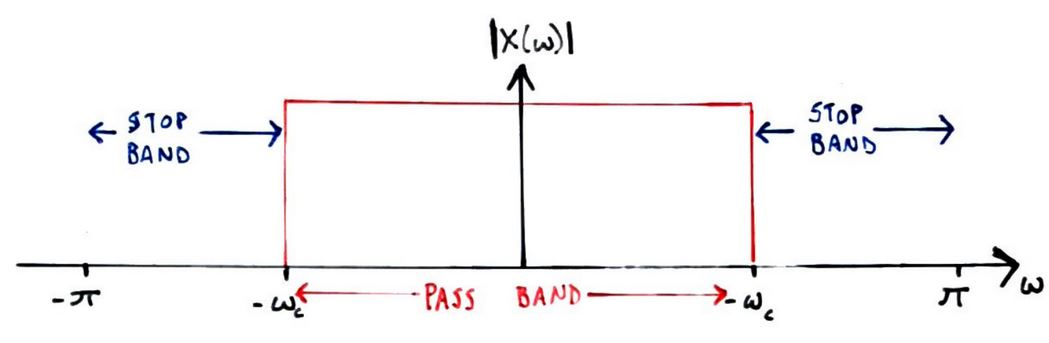
\includegraphics[width=\textwidth]{images/lecture_6_low_pass_filter.JPG}
  \caption{
  }
  \label{fig::lecture_6_low_pass_filter}
\end{figure}
%
There are, however, issues with implementing $h(t)$. For one, it is not causal
since the $\sinc$ is symmetric, and $h(t<0) \neq 0$. It also extends
\textit{ad infinitum} in time, and consequently trucations result in errors.
%
\begin{exmp}
  Consider the impulse response $h(t) =\ex{-at}u(t)$ for $a>0$. We have previously
  found that $\mathscr{F}[h(t)] = \frac{1}{a + \im\omega}$. So,
  %
  \begin{displaymath}
    |H(\omega)| = \sqrt{\frac{1}{(a + \im\omega)(a - \im\omega)}}
    = \frac{1}{\sqrt{a^2 + \omega^2}} \,,
  \end{displaymath}
  %
  which intercepts the vertical axis at $1/a$ and decays like $1/\omega^2$ for
  large $\omega$ -- it resembles a Gaussian. Consequently, $h(t)$ offers
  a fairly crude approximation to a low-pass filter.
\end{exmp}

\subsection{Solving LTI Systems}
%
The most straightforward way to solve a LTI system is to first compute
$X(\omega)$ from $x(t)$, and then multiply it by $H(\omega)$ to yield
$Y(\omega)$. Finally, we perform an inverse Fourier transform to get
$y(t)$.
%
\begin{exmp}
  Consider the signal $x(t) = \ex{-5t}u(t)$ and $h(t) = \ex{-3t}u(t)$.
  Then we have
  %
  \begin{displaymath}
    X(\omega) = \frac{1}{5 + \im\omega} \hspace{10mm}
    H(\omega) = \frac{1}{3 + \im\omega} \,.
  \end{displaymath}
  %
  As a result,
  %
  \begin{align*}
    Y(\omega) &= \frac{1}{(5 + \im\omega)(3 + \im\omega)}
    = \frac{A}{5 + \im\omega} + \frac{B}{3 + \im\omega}
    = \frac{A(3+\im\omega) + B(5+\im\omega)}{(5+\im\omega)(3+\im\omega)} \\
    &= \frac{(3A + 5B) + (A+b)\im\omega}{(5+\im\omega)(3+\im\omega)} \,.
  \end{align*}
  %
  Comparing with out actual expression and equating coefficients, we then
  have $(3A + 5B) = 1, (A + B) = 0$. As such, $A=1/2$ and $B=-1/2$, leading
  us to the output
  %
  \begin{displaymath}
    Y(\omega) = \frac{1}{2(3+\im\omega)} - \frac{1}{2(5+\im\omega)} \,,
  \end{displaymath}
  %
  and since the Fourier transform is linear,
  %
  \begin{displaymath}
    y(t) = \frac{1}{2}\ex{3t}u(t) - \frac{1}{2}\ex{5t}u(t) \,.
  \end{displaymath}
\end{exmp}
%
Fourier techniques can also be used to simplify the solution to differential
equations.
%
\begin{exmp}
  Consider the ODE
  %
  \begin{displaymath}
    \frac{\dsqx{{y}(t)}}{\dx{t}^2} + 4\frac{\dx{y}(t)}{\dx{t}} + 3y(t)
    = \frac{\dx{x}(t)}{\dx{t}} + 2x(t) \,.
  \end{displaymath}
  %
  From the dual $y(t) = x^\prime(t) \Longleftrightarrow Y(\omega) = \im\omega X(\omega)$,
  %
  \begin{displaymath}
    (\im\omega)^2 Y(\omega) + 4\im\omega Y(\omega) + 3Y(\omega)
    = \im\omega X(\omega) + 2X(\omega) \,.
  \end{displaymath}
  %
  Then we can construct the frequency response from the coefficients
  %
  \begin{displaymath}
    H(\omega) = \frac{Y(\omega)}{X(\omega)}
    = \frac{2 + \im\omega}{(1+\im\omega)(3+\im\omega)} \,,
  \end{displaymath}
  %
  which allows us to evaluate $Y(\omega)$ for any $X(\omega)$.
\end{exmp}
